\documentclass[aspectratio=169,10pt]{beamer}

\usetheme{default}
\usecolortheme{default}
\setbeamertemplate{navigation symbols}{}
\setbeamertemplate{footline}[frame number]
\setbeamertemplate{itemize item}{\textbullet}
\setbeamertemplate{itemize subitem}{\textendash}

\definecolor{Ink}{HTML}{1C2430}
\definecolor{Accent}{HTML}{2F5D62}
\definecolor{Warm}{HTML}{8B4D2E}
\definecolor{Rule}{HTML}{D5D9DE}
\definecolor{Wash}{HTML}{F3F5F7}

\setbeamercolor{normal text}{fg=Ink,bg=white}
\setbeamercolor{structure}{fg=Accent}
\setbeamercolor{title}{fg=Ink}
\setbeamercolor{frametitle}{fg=Ink}
\setbeamercolor{author}{fg=Ink}
\setbeamercolor{institute}{fg=Ink}
\setbeamercolor{date}{fg=Ink}
\setbeamerfont{frametitle}{series=\bfseries,size=\large}
\setbeamerfont{title}{series=\bfseries,size=\LARGE}

\usepackage{booktabs}
\usepackage{graphicx}
\usepackage{lmodern}
\usepackage{microtype}
\usepackage{tikz}
\usetikzlibrary{arrows.meta,positioning}
\usepackage[T1]{fontenc}

\setlength{\leftmargini}{1.1em}
\newcommand{\notebox}[1]{%
  \begin{tikzpicture}
    \node[
      fill=Wash,
      draw=Rule,
      line width=0.4pt,
      rounded corners=1.5pt,
      inner xsep=9pt,
      inner ysep=6pt,
      text width=0.92\textwidth,
      align=left,
      font=\footnotesize
    ] {#1};
  \end{tikzpicture}%
}

\begin{document}

%======================================================================
\begin{frame}[plain]
  \vspace{2.6cm}
  \begin{center}
    {\LARGE\bfseries Shen Ruililin\par}
    \vspace{1.1em}
    {\large Laidlaw Scholars\par}
    \vspace{0.55em}
    {\large Bishai Lab\par}
  \end{center}
\end{frame}

%======================================================================
\begin{frame}{Summary}
  \begin{itemize}
    \item Public environmental preparation for a Hong Kong temperature--cardiovascular admissions study covering January 2013--December 2023 is complete at Hong Kong Observatory (HKO) Headquarters.
    \item The monthly exposure file contains mean temperature, mean Tmin, mean Tmax, and official extreme-day counts for $N=132$ months. Annual extreme totals match HKO \textit{Year's Weather} summaries for hot nights, very hot days, and cold days across all 11 years (33/33).
    \item Census and Statistics Department mid-year age--sex population series support person-time denominators, including separate bands for ages 65--69 and 70--74.
    \item Hospital Authority outcome records are not yet available for analysis. Confirmed extract features include ICD-9 coding, patient-level complete admissions, separate older age bands, and exclusion of ED-to-inpatient episodes from the current file.
    \item Near-term analytic focus: merge monthly Tmax/Tmin (and lag temperature) with AMI and stroke admission series; complete Table~1; fit associations only after outcome definition and descriptive quality control.
  \end{itemize}
\end{frame}

%======================================================================
\begin{frame}{Prepared materials and current boundary}
  \begin{columns}[T]
    \begin{column}{0.50\textwidth}
      {\color{Accent}\textbf{Prepared}}
      \begin{itemize}
        \item HKO Headquarters monthly exposure file, 2013--2023
        \item Extreme-day and spell metrics; absolute humidity
        \item Validated annual extremes figure and context note
        \item C\&SD age--sex denominators for rate offsets
        \item Critical literature map and reproducible analysis scripts
      \end{itemize}
    \end{column}
    \begin{column}{0.48\textwidth}
      {\color{Warm}\textbf{Not yet available for inference}}
      \begin{itemize}
        \item Hospital Authority admissions on the analysis account
        \item Confirmed medication and BMI field timing
        \item Real pollution series (placeholder only)
        \item Influenza series for cold-season sensitivity
        \item Any temperature--admission coefficient from real outcomes
      \end{itemize}
    \end{column}
  \end{columns}

  \vspace{0.7em}
  \notebox{\textbf{Boundary.} Environmental descriptives may be shown. Substantive admission associations remain pending secure access and schema confirmation.}
\end{frame}

%======================================================================
\begin{frame}{Monthly temperature, HKO Headquarters, 2013--2023}
  \begin{center}
    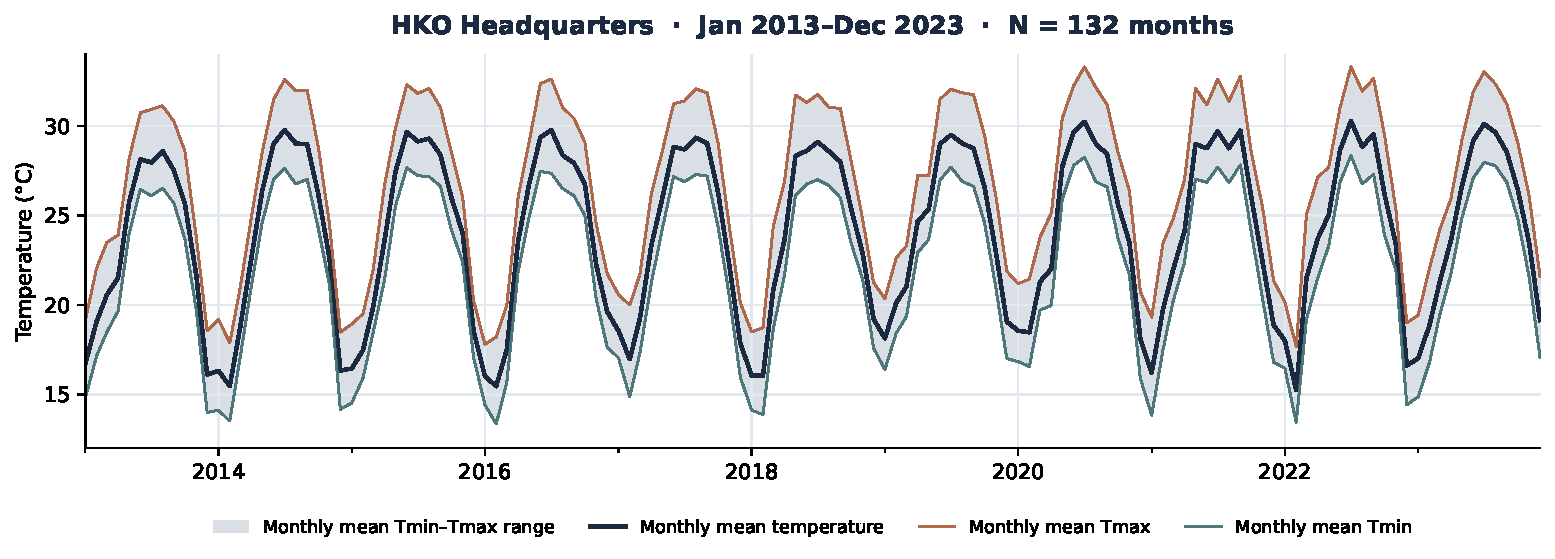
\includegraphics[width=0.94\textwidth]{../../figures/lab_meeting/monthly_temp_ribbon_2013_2023_final.pdf}
  \end{center}
  \vspace{-0.2em}
  \begin{center}
  \scriptsize Environmental exposure only. No admission outcomes.
  \end{center}
\end{frame}

%======================================================================
\begin{frame}{Table~1 shell --- environmental panel complete}
  \begin{columns}[T]
    \begin{column}{0.54\textwidth}
      {\color{Ink}\textbf{Panel A --- Environmental observations}}\\[0.12em]
      {\footnotesize Unit: calendar month \quad $N=132$ \quad HKO Headquarters}

      \vspace{0.35em}
      \footnotesize
      \begin{tabular}{@{}lrr@{}}
        \toprule
        Variable & Mean & SD \\
        \midrule
        Mean temperature ($^\circ$C) & 24.02 & 4.70 \\
        Mean Tmin ($^\circ$C) & 22.10 & 4.69 \\
        Mean Tmax ($^\circ$C) & 26.66 & 4.82 \\
        Hot nights (days/month) & 3.40 & 5.40 \\
        Very hot days (days/month) & 3.19 & 5.18 \\
        Cold days (days/month) & 1.10 & 2.55 \\
        \bottomrule
      \end{tabular}
    \end{column}
    \begin{column}{0.44\textwidth}
      {\color{Ink}\textbf{Panel B --- Admission covariates}}\\[0.12em]
      {\footnotesize Pending Hospital Authority schema and access.}

      \vspace{0.35em}
      \footnotesize
      \begin{itemize}
        \item Age and sex
        \item Diuretics; beta blockers
        \item Metformin; SGLT2 inhibitors
        \item BMI and missingness
      \end{itemize}

      \vspace{0.45em}
      {\footnotesize Model role depends on the at-risk population and whether covariates are measured before the event window.}
    \end{column}
  \end{columns}
\end{frame}

%======================================================================
\begin{frame}{Thermal extremes coexist; cold has not disappeared}
  \begin{center}
    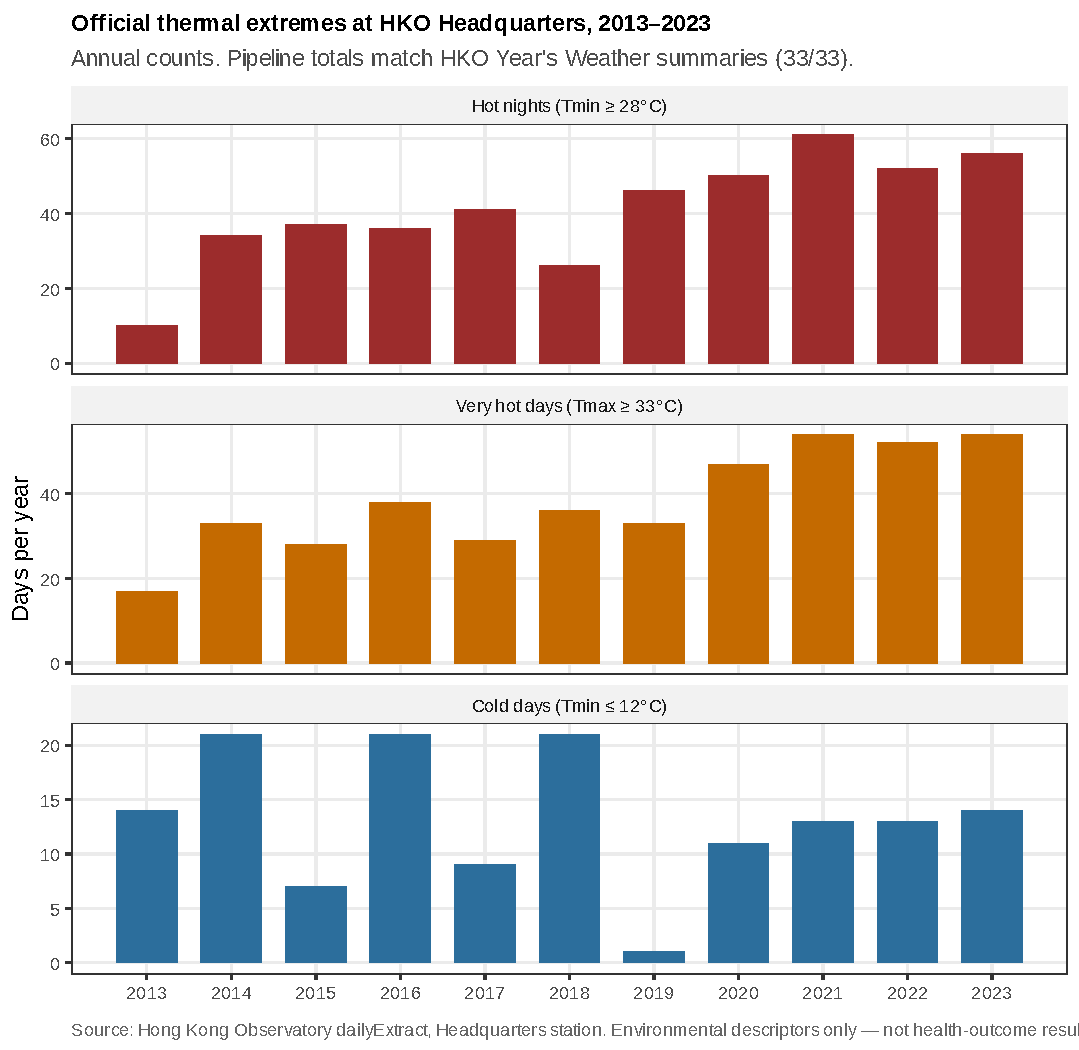
\includegraphics[width=0.78\textwidth,height=0.72\textheight,keepaspectratio]{../../figures/exposure_aging/fig01_annual_extremes_coexistence.pdf}
  \end{center}
  \vspace{-0.15em}
  \begin{center}
  \scriptsize
  Example contrast: 2013 --- 10 hot nights, 14 cold days;
  2021 --- 61 hot nights, 13 cold days.
  Annual totals validated 33/33 against HKO \textit{Year's Weather}.
  \end{center}
\end{frame}

%======================================================================
\begin{frame}{Population aging concentrates person-time in older bands}
  \begin{center}
    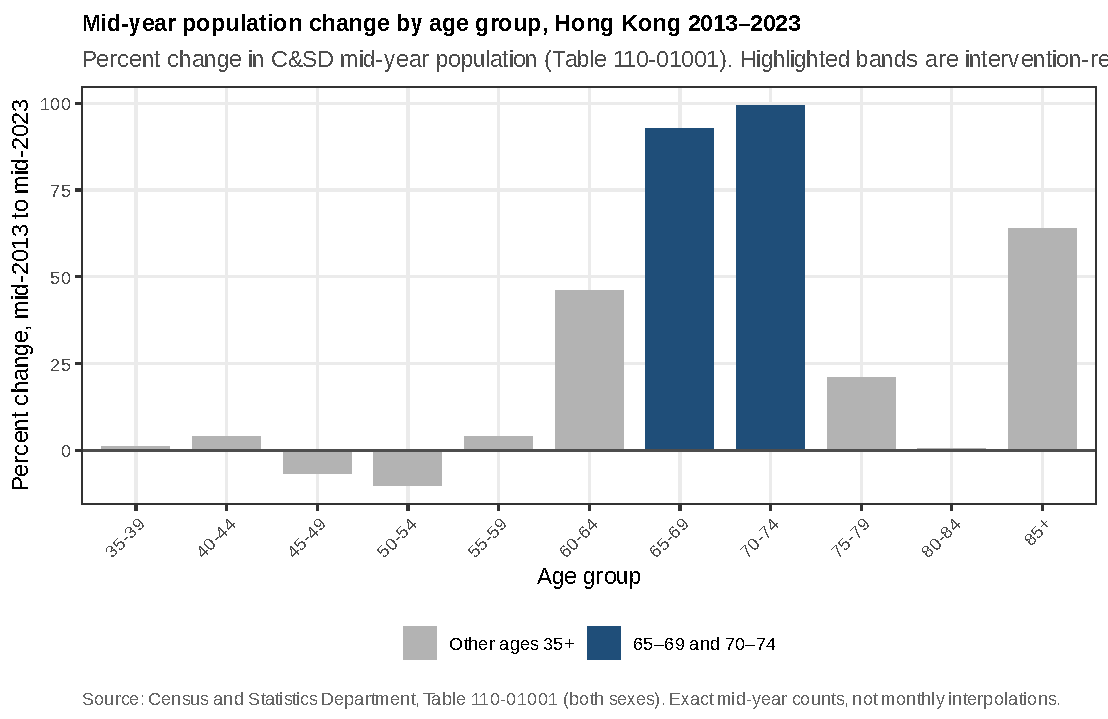
\includegraphics[height=0.62\textheight,keepaspectratio]{../../figures/exposure_aging/fig04_population_aging_pct_change.pdf}
  \end{center}
  \vspace{-0.05em}
  \begin{center}
  \scriptsize
  Mid-year C\&SD series: ages 65--69 rose from 295\,100 (2013) to 568\,500 (2023);
  ages 70--74 from 213\,100 to 424\,800.
  Crude admission counts without age-specific denominators will confound aging with climate.
  \end{center}
\end{frame}

%======================================================================
\begin{frame}{Literature anchors that constrain claims}
  \footnotesize
  \begin{itemize}
    \item \textbf{Goggins et al.\ (2013).} Hong Kong AMI admissions (2000--2009), daily: cooling below $\sim$24$^\circ$C associated with higher AMI ($\sim$3.7\% per 1$^\circ$C, lags 0--13); heat not the dominant finding; NO$_2$ relevant.
    \item \textbf{Goggins et al.\ (2012).} Hemorrhagic and ischemic stroke differ: hemorrhagic stroke shows a strong inverse temperature association (lags 0--4); ischemic stroke weaker and mainly below $\sim$22$^\circ$C (lags 0--13). Subtype separation is required.
    \item \textbf{Guo et al.\ (2024).} Daily hot-season hospitalizations: official binary hot nights (Tmin $\ge$ 28$^\circ$C) not associated with excess risk overall; nighttime heat \emph{intensity} (hot-night excess) was, including circulatory admissions. Binary official counts cannot be treated as self-justifying biology.
    \item \textbf{Wang et al.\ (2019).} Consecutive extremely hot weather events (including multi-day hot nights and combined day--night patterns) raise mortality risk; event structure matters beyond raw monthly totals.
    \item \textbf{Guo et al.\ (2025); Yang et al.\ (2025).} Pollution can modify temperature--hospitalization associations; cold and influenza jointly relate to stroke admissions at weekly scale.
  \end{itemize}
\end{frame}

%======================================================================
\begin{frame}{Implications for design and interpretation}
  \begin{itemize}
    \item \textbf{Trigger versus burden.} Daily distributed-lag models estimate acute triggering. Monthly models estimate hospital-burden associations. Coefficients are not interchangeable with historical per-$^\circ$C daily estimates.
    \item \textbf{Cold remains co-primary.} A heat-only narrative is inconsistent with local historical evidence and with continued cold-day occurrence in high-heat years.
    \item \textbf{Official extremes versus intensity.} Monthly hot-night counts remain policy-aligned; spell and intensity-style alternatives are scientific checks. A null official-count association would be compatible with Guo et al.\ (2024).
    \item \textbf{Novelty discipline.} Claims of being the first Hong Kong temperature--CVD or hot-night hospitalization study are not defensible.
    \item \textbf{Near-term exposure emphasis.} Supervisory guidance directs the first merge toward monthly Tmax/Tmin and lag temperature for AMI and stroke admission risk, with extreme-day metrics retained as secondary specifications.
  \end{itemize}
\end{frame}

%======================================================================
\begin{frame}{Working hypotheses (prespecified; untested on real outcomes)}
  \begin{enumerate}
    \item Colder monthly conditions, and higher cold-day counts, associate with higher AMI and ischemic-stroke admission rates.
    \item Higher monthly Tmax/Tmin, or heat-extreme burden, may associate with admissions, especially in older age bands; null findings for official binary hot nights remain scientifically interpretable.
    \item Associations differ across AMI, ischemic stroke, and hemorrhagic stroke.
    \item Age and clinical covariates (medications, BMI), when measured with valid pre-event timing, may modify temperature--admission associations.
    \item Pollution and influenza adjustments are staged sensitivities, not prerequisites for the first descriptive Hospital Authority report.
  \end{enumerate}
\end{frame}

%======================================================================
\begin{frame}{Analysis unit: one schema fork}
  \footnotesize
  Does the extract contain admissions only, or a defined cohort with non-event follow-up?

  \vspace{0.45em}
  {\color{Ink}\textbf{Default for the first analysis (admissions-only)}}
  \vspace{0.25em}

  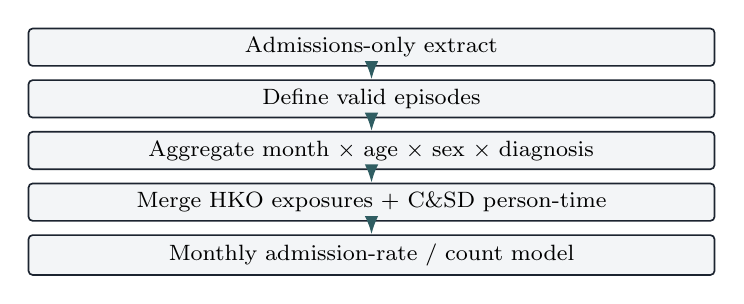
\begin{tikzpicture}[
    node distance=0.16cm,
    box/.style={
      draw=Ink, line width=0.6pt, rounded corners=1.5pt,
      align=center, font=\footnotesize, inner sep=3.2pt,
      text width=0.70\textwidth, fill=Wash
    },
    arr/.style={-{Latex}, thick, Accent}
  ]
    \node[box] (a) {Admissions-only extract};
    \node[box, below=of a] (b) {Define valid episodes};
    \node[box, below=of b] (c) {Aggregate month $\times$ age $\times$ sex $\times$ diagnosis};
    \node[box, below=of c] (d) {Merge HKO exposures + C\&SD person-time};
    \node[box, below=of d] (e) {Monthly admission-rate / count model};
    \draw[arr] (a) -- (b);
    \draw[arr] (b) -- (c);
    \draw[arr] (c) -- (d);
    \draw[arr] (d) -- (e);
  \end{tikzpicture}

  \vspace{0.35em}
  \footnotesize
  Alternative only if non-event follow-up exists: patient-month risk model.
  Until the denominator is confirmed, language should refer to monthly admission counts or rates, not patient-level risk.
\end{frame}

%======================================================================
\begin{frame}{Temperature variables and lag sequence}
  \begin{columns}[T]
    \begin{column}{0.52\textwidth}
      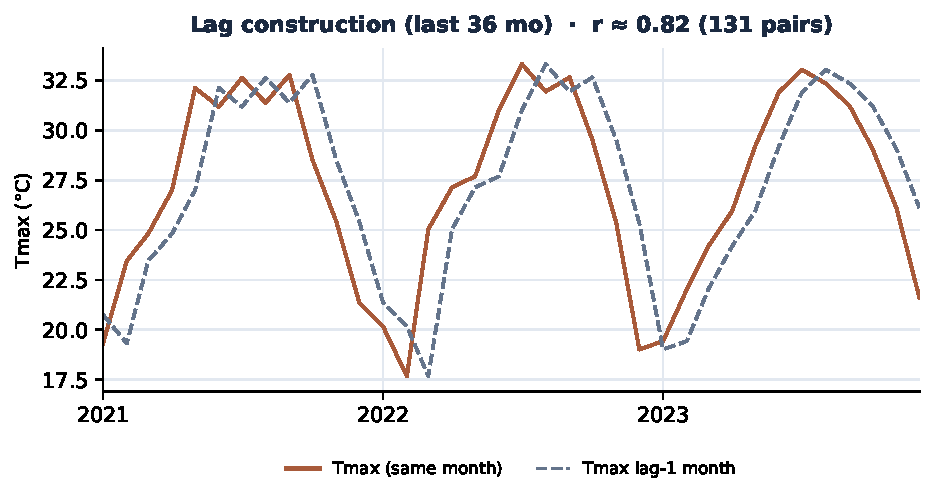
\includegraphics[width=\textwidth]{../../figures/lab_meeting/tmax_lag1_example_final.pdf}
    \end{column}
    \begin{column}{0.46\textwidth}
      \footnotesize
      \begin{itemize}
        \item Analysis file can carry same-month and lag-1 mean, Tmin, and Tmax.
        \item Same-month versus lag-1 mean Tmax: $r=0.8225$ ($n=131$ pairs).
        \item Fit temperature specifications separately; avoid one saturated model.
        \item Proposed sequence: same-month initial; lag-1 sensitivity; mean of current and previous month as secondary.
        \item Extend processed weather through December 2012 so January 2013 has valid lag-1.
      \end{itemize}
    \end{column}
  \end{columns}
\end{frame}

%======================================================================
\begin{frame}{Confirmations required before the first outcome report}
  \footnotesize
  \begin{enumerate}
    \item Meaning of ``DAE records included'' in the ICD-9 extract.
    \item Row/episode unit; principal versus any-position diagnosis; transfer and recurrence rules.
    \item Whether the extract is admissions-only or a cohort with non-event months.
    \item Presence and timing of diuretics, beta blockers, metformin, SGLT2 inhibitors, and BMI.
    \item Primary temperature metric for the first model (mean, Tmin/Tmax, or extreme-day counts as secondary).
    \item Access pathway timing (authorization signatures and secure-server onboarding).
    \item Whether an ethics-protocol amendment is required for this Hospital Authority use.
  \end{enumerate}

  \vspace{0.55em}
  \notebox{\textbf{Next deliverable after access and schema confirmation:} validated data dictionary and quality-control report; descriptive admission counts and age-specific rates; completed Table~1. Regression begins only after outcome definition and descriptive quality control are approved.}
\end{frame}

\end{document}
